% fig4a-ged-matrix.tex
\documentclass[tikz,border=5pt]{standalone}
% common-styles.tex
% Shared TikZ styles for wonton-proof paper figures

\usepackage{silence}
\WarningFilter{latex}{Missing character} 
\tracinglostchars=0 % Suppress engine-level "Missing character" warnings

\usepackage{fontspec}
\usepackage{unicode-math}

% Use filenames for reliability with Tectonic
\setmainfont{LibertinusSerif-Regular.otf}[
    BoldFont=LibertinusSerif-Bold.otf,
    ItalicFont=LibertinusSerif-Italic.otf,
    BoldItalicFont=LibertinusSerif-BoldItalic.otf
]
\setsansfont{LibertinusSans-Regular.otf}[
    BoldFont=LibertinusSans-Bold.otf,
    ItalicFont=LibertinusSans-Italic.otf
]
\setmonofont{LibertinusMono-Regular.otf}

% Try a more standard math font if LibertinusMath is causing nullfont issues
\setmathfont{LibertinusMath-Regular.otf}
% \setmathfont{latinmodern-math.otf}[range=digits] 

\usepackage{amsmath}
\usepackage{tikz}
\usepackage{forest}

\usetikzlibrary{
    arrows.meta,
    calc,
    decorations.pathreplacing,
    fit,
    positioning,
    shapes.geometric,
    shapes.misc,
    backgrounds,
    shadows.blur,
    fadings
}

% Color palette (muted, print-friendly)
\definecolor{ink}{RGB}{45,45,52}
\definecolor{muted}{RGB}{115,115,125}
\definecolor{highlight}{RGB}{198,120,44}
\definecolor{accentblue}{RGB}{86,130,178}
\definecolor{accentgreen}{RGB}{84,156,132}
\definecolor{blocked}{RGB}{140,75,75}
\definecolor{goalnode}{RGB}{255,255,255}
\definecolor{terminal}{RGB}{238,239,244}
\definecolor{deadnode}{RGB}{248,245,245}
\definecolor{flowbox}{RGB}{250,250,252}
\definecolor{basin1}{RGB}{224,234,248}
\definecolor{basin2}{RGB}{246,232,221}
\definecolor{basin3}{RGB}{228,242,234}
\definecolor{heatbase}{RGB}{86,130,178}

\tikzset{
    line cap=round,
    line join=round,
    pop/.style={
        blur shadow={shadow blur steps=5, shadow blur extra rounding=1.3pt}
    },
    base node/.style={
        rounded rectangle,
        draw=ink,
        line width=0.6pt,
        fill=goalnode,
        text=ink,
        minimum width=2.2cm,
        minimum height=0.7cm,
        align=center,
        pop
    },
    goal/.style={base node, fill=goalnode},
    terminal/.style={base node, fill=terminal, line width=0.9pt},
    dead/.style={base node, fill=deadnode, dashed},
    flowbox/.style={
        rectangle,
        draw=muted,
        rounded corners=3pt,
        fill=flowbox,
        minimum width=1.8cm,
        minimum height=0.6cm,
        align=center,
        font=\normalfont\small,
        text=ink,
        pop
    },
    decision/.style={
        diamond,
        draw=muted,
        fill=flowbox,
        aspect=2.4,
        font=\normalfont\small,
        inner sep=1pt,
        text=ink
    },
    protocolbox/.style={
        rectangle,
        draw=muted,
        rounded corners=4pt,
        fill=flowbox,
        minimum width=2cm,
        minimum height=0.8cm,
        font=\normalfont\small,
        align=center,
        text=ink
    },
    tactic/.style={
        ->,
        >=Stealth,
        draw=muted,
        line width=0.75pt
    },
    tacticlight/.style={
        ->,
        >=Stealth,
        draw=muted!45,
        dashed,
        line width=0.6pt
    },
    backprop/.style={
        ->,
        >=Stealth,
        draw=muted!70,
        dashed,
        line width=0.6pt
    },
    selected/.style={
        tactic,
        draw=highlight,
        line width=1.4pt
    },
    divergetactic/.style={
        tactic,
        draw=highlight,
        line width=1.4pt
    },
    divergenode/.style={
        base node,
        draw=highlight,
        line width=1.0pt
    },
    divergeblock/.style={
        blockedtactic,
        line width=1.2pt
    },
    blockedtactic/.style={
        tactic,
        draw=blocked,
        densely dashed
    },
    flowarrow/.style={
        ->,
        >=Stealth,
        draw=muted,
        line width=0.75pt
    },
    crosslink/.style={
        -,
        draw=muted!70,
        dotted,
        line width=0.6pt
    },
    annot/.style={
        font=\normalfont\footnotesize,
        text=muted
    },
    visit/.style={
        annot,
        font=\normalfont\scriptsize
    },
    annotbg/.style={
        annot,
        fill=white,
        inner sep=1.5pt
    },
    tacticlabel/.style={
        annot,
        font=\ttfamily\footnotesize,
        text=muted
    },
    formula/.style={
        font=\normalfont\footnotesize,
        draw=muted,
        rounded corners=2pt,
        fill=white,
        inner sep=3pt
    },
    paneltitle/.style={
        font=\normalfont\bfseries,
        text=ink
    },
    trajectory/.style={
        ->,
        draw=muted!70,
        line width=0.6pt
    }
}

\begin{document}
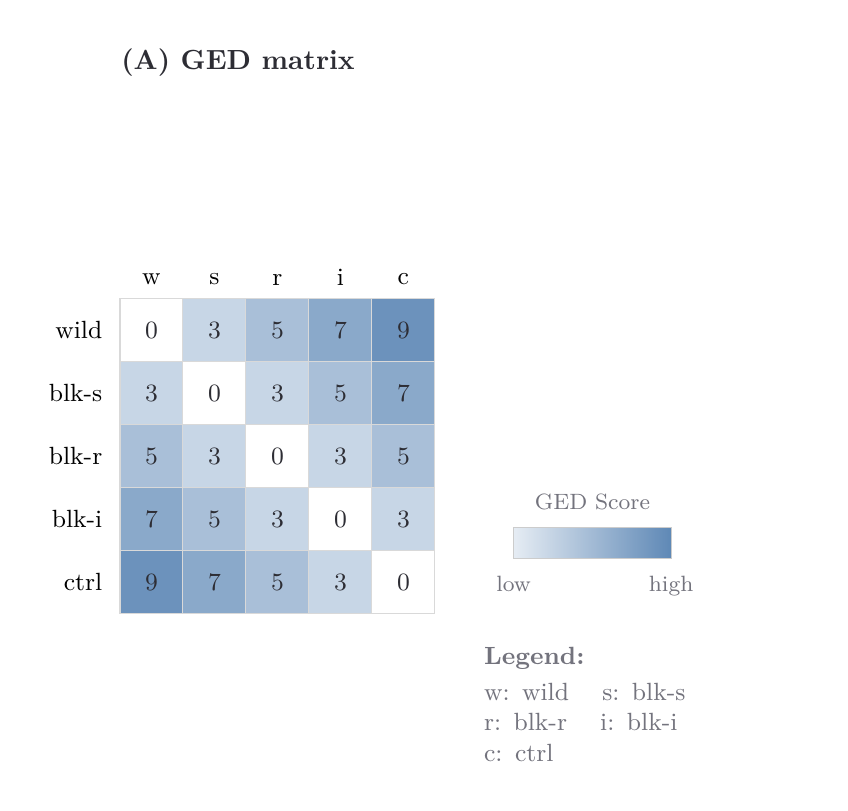
\begin{tikzpicture}[
    every node/.style={font=\small},
    show background rectangle,
    background rectangle/.style={fill=white}
]
\tikzset{cell/.style={draw=black!15, line width=0.4pt}}

\begin{scope}[shift={(0, 0)}]
    \node[paneltitle, anchor=south] at (1.5, 3.5) {(A) GED matrix};
    \def\cellsize{0.8} % Larger cells

    % Matrix cells
    \foreach \i in {0,1,2,3,4} {
        \foreach \j in {0,1,2,3,4} {
            \ifnum\i=\j
                \fill[white] (\j*\cellsize, -\i*\cellsize) rectangle +(\cellsize, \cellsize);
                \node[font=\small, text=ink] at (\j*\cellsize + 0.5*\cellsize, -\i*\cellsize + 0.5*\cellsize) {0};
            \else
                % Fake data for illustration
                \pgfmathtruncatemacro{\dist}{abs(\i-\j)}
                \pgfmathtruncatemacro{\val}{\dist * 2 + 1}
                \pgfmathsetmacro{\shade}{15 + \dist*18}
                \fill[heatbase!\shade!white] (\j*\cellsize, -\i*\cellsize) rectangle +(\cellsize, \cellsize);
                \node[font=\small, text=ink] at (\j*\cellsize + 0.5*\cellsize, -\i*\cellsize + 0.5*\cellsize) {\val};
            \fi
            \draw[cell] (\j*\cellsize, -\i*\cellsize) rectangle +(\cellsize, \cellsize);
        }
    }

    % Row labels
    \foreach \i/\lbl in {0/wild,1/blk-s,2/blk-r,3/blk-i,4/ctrl} {
        \node[anchor=east, font=\small, align=right] at (-0.1, -\i*\cellsize + 0.5*\cellsize) {\lbl};
    }

    % Column labels (abbreviated)
    \foreach \j/\lbl in {0/w,1/s,2/r,3/i,4/c} {
        \node[anchor=south, font=\small] at (\j*\cellsize + 0.5*\cellsize, \cellsize + 0.05) {\lbl};
    }

    % Colorbar
    \begin{scope}[shift={(5.0, -2.5)}]
        \shade[left color=heatbase!15!white, right color=heatbase!95!white] (0,0) rectangle (2.0, 0.4);
        \draw[black!20] (0, 0) rectangle (2.0, 0.4);
        
        \node[anchor=north, font=\footnotesize, text=muted] at (0, -0.1) {low};
        \node[anchor=north, font=\footnotesize, text=muted] at (2.0, -0.1) {high};
        \node[anchor=south, font=\footnotesize, text=muted] at (1.0, 0.5) {GED Score};

        % Legend
        \node[annot, anchor=north west, text width=4cm, font=\small, align=left] at (-0.5, -1.0)
            {\textbf{Legend:}\\[2pt]
            w: wild \quad s: blk-s\\
            r: blk-r \quad i: blk-i\\
            c: ctrl};
    \end{scope}
\end{scope}
\end{tikzpicture}
\end{document}